\documentclass[12pt]{scrartcl}

\usepackage[sectionmark,nodate,cs,epi,bib,hints]{bubu}
\addbibresource{refs.bib}

%%%%%%%%%%%%%%%%%%%%%%%%%%%%%%%%%%%%%%%%%%%%%%%%%%%%%%%%%%%%%%%%%%%%%%%

\title{LaTeX Template}
\author{Avigyan Chakraborty}
\date{Last Updated: \today}

\begin{document}

\maketitle

\epigraph{Is it that you're being good to-get-her, or that you think you're good together?}{Me (inspired by “Good Together” --- Shy Martin)}

\tableofcontents

\newpage


\section{\texttt{mdthm} Environments}


This is the color of the default \textbf{bold text}.

\begin{definition}
[Name]
This is a Definition.
\end{definition}

\begin{theorem}
[Name]
This is a Theorem.
\end{theorem}

\begin{lemma}
[Name]
This is a Lemma.
\end{lemma}

\begin{corollary}
[Name]
This is a Corollary.
\end{corollary}

\begin{proposition}
[Name]
This is a Proposition.
\end{proposition}

\begin{assume}
[Name]
This is an Assumption.
\end{assume}

\begin{conjecture}
[Name]
This is a Conjecture.
\end{conjecture}

\begin{fact}
[Name]
This is a Fact.
\end{fact}

\begin{ques}
[Name]
This is a Question.
\end{ques}

\begin{answer}
[Name]
This is an Answer.
\end{answer}

\begin{exercise}
[Name]
This is an Exercise.
\end{exercise}
\begin{hints}
  \begin{hint}
    First hint.
  \end{hint}
\end{hints}

\begin{problem}
[Name]
This is a Problem.
\end{problem}
\begin{hints}
  \begin{hint}
    First hint.
  \end{hint}
  \begin{hint}
    Second hint.
  \end{hint}
\end{hints}

\begin{algorithm}
[Name]
This is an Algorithm.
\end{algorithm}

\begin{claim}
[Name]
This is a Claim.
\end{claim}

\begin{proof}
This is a Proof.
\end{proof}

\begin{example}
[Name]
This is an Example.
\end{example}

\begin{soln}
This is a Solution.
\end{soln}

\hrulebar

\begin{proof}
This is a Proof.
\end{proof}

\begin{soln}
This is a Solution.
\end{soln}

\begin{proof}
This is a Proof.
\end{proof}

\begin{soln}
This is a Solution.
\end{soln}

\begin{remark}
[Name]
  This is a Remark.\footnote{This is footnote for this remark.}
\end{remark}

\newpage

\section{Other Environments}


\begin{table}[htbp]
\label{tab:1}
\centering
\begin{tabular}{||c c c||}

\hline
Col1 & Col2 & Col3 \\ [0.5ex]
\hline\hline

1 & 2 & 3 \\
\hline

\end{tabular}
\caption{This is a table}
\end{table}

\begin{enumerate}[(a)]
  \ii First.
  \ii Second.
\end{enumerate}

\begin{itemize}
  \ii First.
  \ii Second.
\end{itemize}

\begin{figure}[htbp]
    \centering
    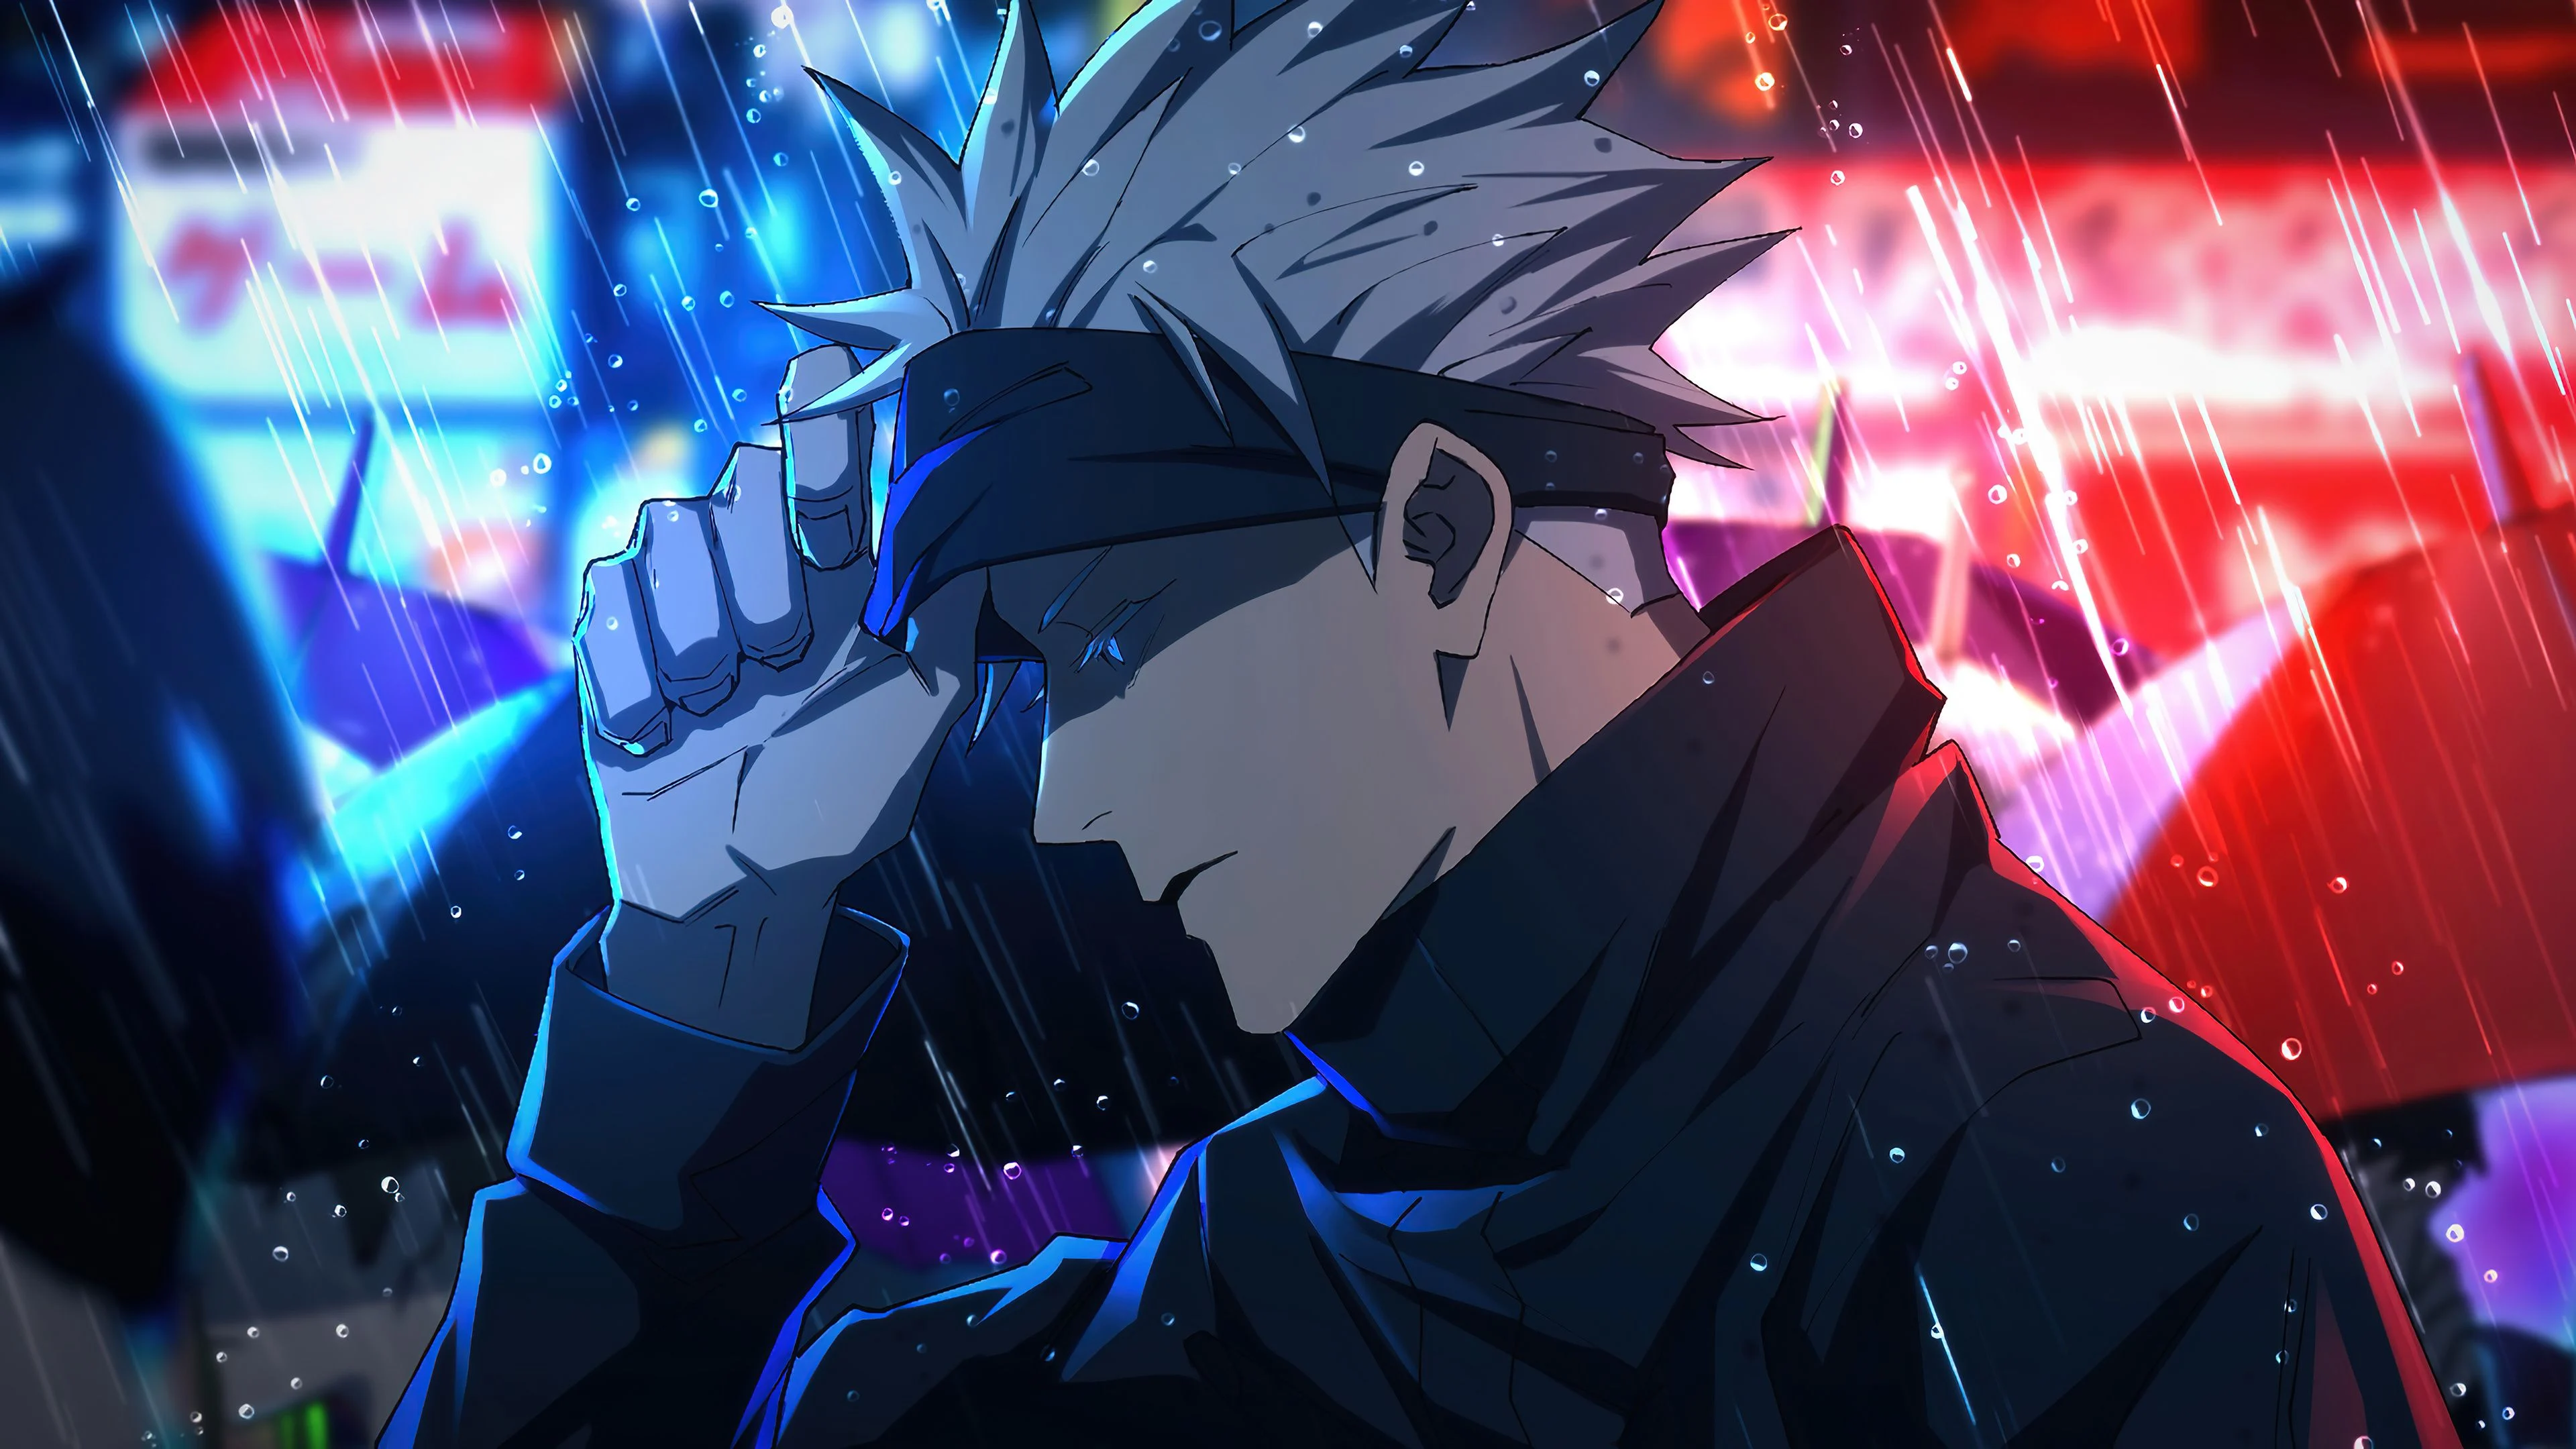
\includegraphics[width=0.5\textwidth,keepaspectratio]{images/gojo_pfp.png}
    % height=\textheight does what it's expected to do similarly as well
    \caption{Cool Gojo 4K Wallpaper}
    \label{fig:gojo1}
\end{figure}

\newpage

\section{Math Environments}


\begin{align*}
  x^2
  &= \frac{2x^2}{2}\\
  &= \frac{(x+1)^2+(x-1)^2 - 2}{2}
.\end{align*}

\[
  f(x)=\begin{cases}
    0, & \text{if } x \text{ is rational} \\
    1, & \text{otherwise}
  .\end{cases}
\]

\[
  g(x)=\begin{cases}
    0, & \text{if } x \text{ is irrational}\\
    \frac{1}{q}, & \text{if } x=\frac{p}{q}
    \text{ where $p$, $q$ are integers with $\gcd(p,q)=1$}.
  \end{cases}
.\]

\[
\sin \cos \tan \csc \sec \cot \arcsin \arccos \arctan \arccsc \arcsec \arccot
.\]

\[
\vp{p}{p^2} = 2 \text{ and } \Pow{\odot(ABC)}{A} = 0
.\]

\[
  \iint\limits_{x^2+y^2\le 1} (x+y)\mathrm{d}x \mathrm{d}y = 0
.\]

\[
  \int_{0}^{1} \ln(x) = -1
.\]

\[
\dd[n]{f}{x} \pd[n]{f}{x}
.\]


\newpage

\section{CS and ASY Environments}


\begin{figure}[htbp]
  \centering
  \begin{asy}
    pair A = (-57.30375,53.83617);
    pair B = (-83.34998,-39.17961);
    pair C = (43.19882,-39.61374);
    pair H = (-57.62315,-39.26787);
    pair D = (-31.07334,-39.35895);
    pair L = (-70.32686,7.32827);
    pair K = (-7.05246,7.11121);
    pair P = (-20.20788,-77.96332);
    pair X = (-22.03030,7.16259);
    pair Y = (61.56501,6.87581);
    pair M = (-44.18855,7.23860);
    pair I = (-40.28433,-6.63285);
    pair E = (-69.06976,-22.25320);
    pair F = (-23.36015,-3.92844);
    import graph;
    size(8cm);
    pen dps = linewidth(0.5) + fontsize(13); defaultpen(dps);
    real xmin = -130, xmax = 85, ymin = -100, ymax = 85;
    draw(A--B, linewidth(0.5));
    draw(B--C, linewidth(0.5));
    draw(C--A, linewidth(0.5));
    draw(circle((-19.96366,-6.77439), 71.18934), linewidth(0.5));
    draw(circle(L, 48.29685), linewidth(0.5) + blue);
    draw(circle(K, 68.61788), linewidth(0.5) + blue);
    draw(circle(P, 74.10196), linewidth(0.5) + linetype("4 4") + red);
    draw(B--M, linewidth(0.5) + red);
    draw(M--C, linewidth(0.5) + red);
    draw(A--P, linewidth(0.5));
    draw(H--A, linewidth(0.5));
    draw(L--Y, linewidth(0.5));
    dot("$A$", A, N);
    dot("$B$", B, SW);
    dot("$C$", C, SE);
    dot("$H$", H, dir(270));
    dot("$D$", D, SE);
    dot("$L$", L, NW);
    dot("$K$", K, NE);
    dot("$P$", P, dir(270));
    dot("$X$", X, NW);
    dot("$Y$", Y, NE);
    dot("$M$", M, NW);
    dot("$I$", I, NW);
    dot("$E$", E, NW);
    dot("$F$", F, NE);
    clip((xmin,ymin)--(xmax,ymin)--(xmax,ymax)--(xmin,ymax)--cycle);
  \end{asy}
  \caption{An asy diagram}
  \label{fig:asy1}
\end{figure}

\begin{minted}{python}
  import numpy as np
      
  def incmatrix(genl1,genl2):
      m = len(genl1)
      n = len(genl2)
      M = None #to become the incidence matrix
      VT = np.zeros((n*m,1), int)  #dummy variable
      
      #compute the bitwise xor matrix
      M1 = bitxormatrix(genl1)
      M2 = np.triu(bitxormatrix(genl2),1) 

      for i in range(m-1):
          for j in range(i+1, m):
              [r,c] = np.where(M2 == M1[i,j])
              for k in range(len(r)):
                  VT[(i)*n + r[k]] = 1;
                  VT[(i)*n + c[k]] = 1;
                  VT[(j)*n + r[k]] = 1;
                  VT[(j)*n + c[k]] = 1;
                  
                  if M is None:
                      M = np.copy(VT)
                  else:
                      M = np.concatenate((M, VT), 1)
                  
                  VT = np.zeros((n*m,1), int)
      
      return M
\end{minted}

\newpage

\section{Hints}


\printhint

\newpage

\section{Bibliography}


Random text for citing some document in my \LaTeX\ file \cite{knuth1997}.

\printbibliography


\end{document}
